\documentclass[12pt, a4paper]{article}
\usepackage[a4paper, top=2.5cm, bottom=2.5cm, left=2cm, right=2cm]{geometry}
\usepackage{fontspec}
\usepackage{polyglossia}
\setmainlanguage{vietnamese}
\setotherlanguage{english}

\IfFontExistsTF{Times New Roman}{
    \setmainfont{Times New Roman}
}{
    \setmainfont{TeX Gyre Termes}
}

\usepackage{enumitem}
\setlist[itemize]{label=-}

\usepackage{amsmath, amssymb, amsfonts}
\usepackage{graphicx}
\usepackage{float}
\usepackage{algorithm}
\usepackage{algpseudocode}
\usepackage{booktabs}
\usepackage{hyperref}
\usepackage{listings}
\usepackage{xcolor}

\definecolor{codegreen}{rgb}{0,0.6,0}
\definecolor{codegray}{rgb}{0.5,0.5,0.5}
\definecolor{codepurple}{rgb}{0.58,0,0.82}
\definecolor{backcolour}{rgb}{0.95,0.95,0.92}
\lstdefinestyle{mystyle}{
    backgroundcolor=\color{backcolour},
    commentstyle=\color{codegreen},
    keywordstyle=\color{magenta},
    numberstyle=\tiny\color{codegray},
    stringstyle=\color{codepurple},
    basicstyle=\ttfamily\footnotesize,
    breaklines=true, captionpos=b, keepspaces=true,
    numbers=left, numbersep=5pt,
    showspaces=false, showstringspaces=false,
    showtabs=false, tabsize=4
}
\lstset{style=mystyle}

\title{\textbf{BÁO CÁO TIẾN ĐỘ: ĐÁNH GIÁ TRAVERSABILITY ĐA PHƯƠNG PHÁP VÀ TÍCH HỢP HỆ THỐNG QUY HOẠCH 2.5D}}
\author{Nhóm 3: Động lực học \& Điều khiển}
\date{Ngày 19 tháng 5, 2026}

\begin{document}

\maketitle

\begin{abstract}
Báo cáo này trình bày các kết quả nghiên cứu bổ sung kể từ báo cáo lần 1 (28/04/2026) của Nhóm 3. Nhóm đã mở rộng hệ thống quy hoạch đường đi 2.5D bằng cách \textbf{tích hợp thêm ba lớp đánh giá Traversability} (Hình học -- Geometric, Vật lý -- Physical, Ngữ nghĩa -- Semantic) vào pipeline tổng thể, đồng thời củng cố kết quả thực nghiệm A* và NMPC bằng các bảng số liệu chi tiết hơn. Toàn bộ mã nguồn Python được lưu tại thư mục \texttt{3. code} của dự án.
\end{abstract}

% ============================================================
\section{Tóm tắt tiến độ từ báo cáo lần 1 (28/04/2026)}
% ============================================================

Nhóm 3 đã hoàn thiện các nội dung sau kể từ báo cáo lần 1:

\begin{enumerate}
    \item \textbf{Đã hoàn thiện (từ báo cáo lần 1):}
    \begin{itemize}
        \item Hàm chi phí tổng hợp Bekker-Wong + Minetti + LTR tích hợp vào Weighted A*
        \item Thực nghiệm đối chiếu 5 thuật toán (PRM, BIT*, FMM, HPA*, ACO -- đều thất bại)
        \item Bộ điều khiển NMPC (CasADi/IPOPT) bám quỹ đạo A* dưới nhiễu trượt $10\%$
    \end{itemize}
    \item \textbf{Bổ sung trong báo cáo này (19/05/2026):}
    \begin{itemize}
        \item Phân tích Traversability đa phương pháp: Geometric + Physical + Semantic + Fusion
        \item Bộ figure tổng hợp mới: biểu đồ cột 5 thuật toán, hàm chi phí Minetti, sơ đồ kiến trúc
        \item Bảng số liệu đầy đủ cho cả 3 nội dung chính
        \item Định hướng tích hợp lên ROS 2 và nâng cấp ACADOS/MCTD
    \end{itemize}
\end{enumerate}

% ============================================================
\section{Đánh giá Traversability Đa phương pháp (Bổ sung mới)}
% ============================================================

Trả lời cho yêu cầu của bài survey về \textit{``Phân loại các phương pháp đánh giá Traversability''}, nhóm đã nghiên cứu và triển khai thực nghiệm số ba lớp phương pháp bổ sung lẫn nhau \cite{triebel2006}.

\subsection{Phương pháp Hình học (Geometric Traversability)}

Nhóm trích xuất ba đặc trưng hình học thuần túy từ dữ liệu độ cao của BenchNav \cite{endo2024}:

\begin{itemize}
    \item \textbf{Độ dốc (Slope):} $|\nabla h| = \sqrt{(\partial h/\partial x)^2 + (\partial h/\partial y)^2}$ -- ngưỡng an toàn $< 30^\circ$
    \item \textbf{Độ gồ ghề (Roughness):} Độ lệch chuẩn độ cao trong cửa sổ $5 \times 5$ ô xung quanh
    \item \textbf{Chướng ngại bậc (Step hazard):} Chênh lệch độ cao cực đại trong cửa sổ $3 \times 3$ ô
\end{itemize}

Công thức tổng hợp (trọng số thực nghiệm $w_s = 0.5$, $w_r = 0.3$, $w_h = 0.2$):
\begin{equation}
    T_{\text{geo}} = 1 - \bigl(w_s \cdot s_{\text{norm}} + w_r \cdot r_{\text{norm}} + w_h \cdot h_{\text{norm}}\bigr) \in [0, 1]
\end{equation}
Kết quả: điểm trung bình $\bar{T}_{\text{geo}} = 0.612$, $\approx 18\%$ diện tích bản đồ nguy hiểm.

\subsection{Phương pháp Vật lý (Physical Traversability)}

Dựa trên mô hình Terramechanics Bekker-Wong \cite{bekker1956} và điều kiện ma sát Coulomb \cite{higa2019}:

\textbf{Điều kiện không trượt:} $\mu(\text{class}) \geq \tan(\theta_{\text{slope}})$, trong đó hệ số ma sát $\mu$ theo loại đất:
\begin{itemize}
    \item Class 0 (Cỏ/Grass): $\mu = 0.65$ \quad Class 1 (Bùn/Mud): $\mu = 0.20$
    \item Class 2 (Đá/Rock): $\mu = 0.80$ \quad Class 3 (Cát/Sand): $\mu = 0.40$
\end{itemize}

\begin{equation}
    T_{\text{phys}} = \text{clip}\!\left(\frac{\mu(\text{class}) - \tan(\theta_{\text{slope}})}{\mu(\text{class})},\; 0,\; 1\right)
\end{equation}
Kết quả: điểm trung bình $\bar{T}_{\text{phys}} = 0.573$, $\approx 22\%$ diện tích nguy hiểm (nghiêm khắc nhất do vùng bùn).

\subsection{Phương pháp Ngữ nghĩa (Semantic Traversability)}

Trong thực tế, mạng CNN phân loại loại đất từ ảnh RGB + LiDAR \cite{jiang2021rellis}. Nhóm mô phỏng đầu ra của mạng CNN bằng cách gán điểm traversability theo nhãn lớp đất đã biết, có thêm nhiễu Gaussian ($\sigma = 0.05$) để mô phỏng uncertainty của mô hình học máy:

\begin{itemize}
    \item Grass ($T = 0.90$), Mud ($T = 0.20$), Rock ($T = 0.60$), Sand ($T = 0.55$)
\end{itemize}

Kết quả: điểm trung bình $\bar{T}_{\text{sem}} = 0.643$, $\approx 15\%$ diện tích nguy hiểm.

\subsection{Fusion đa phương pháp và Kết quả tổng hợp}

Ba phương pháp được tích hợp bằng weighted fusion:
\begin{equation}
    T_{\text{fused}} = 0.35\,T_{\text{geo}} + 0.35\,T_{\text{phys}} + 0.30\,T_{\text{sem}}
\end{equation}

\begin{figure}[H]
  \centering
  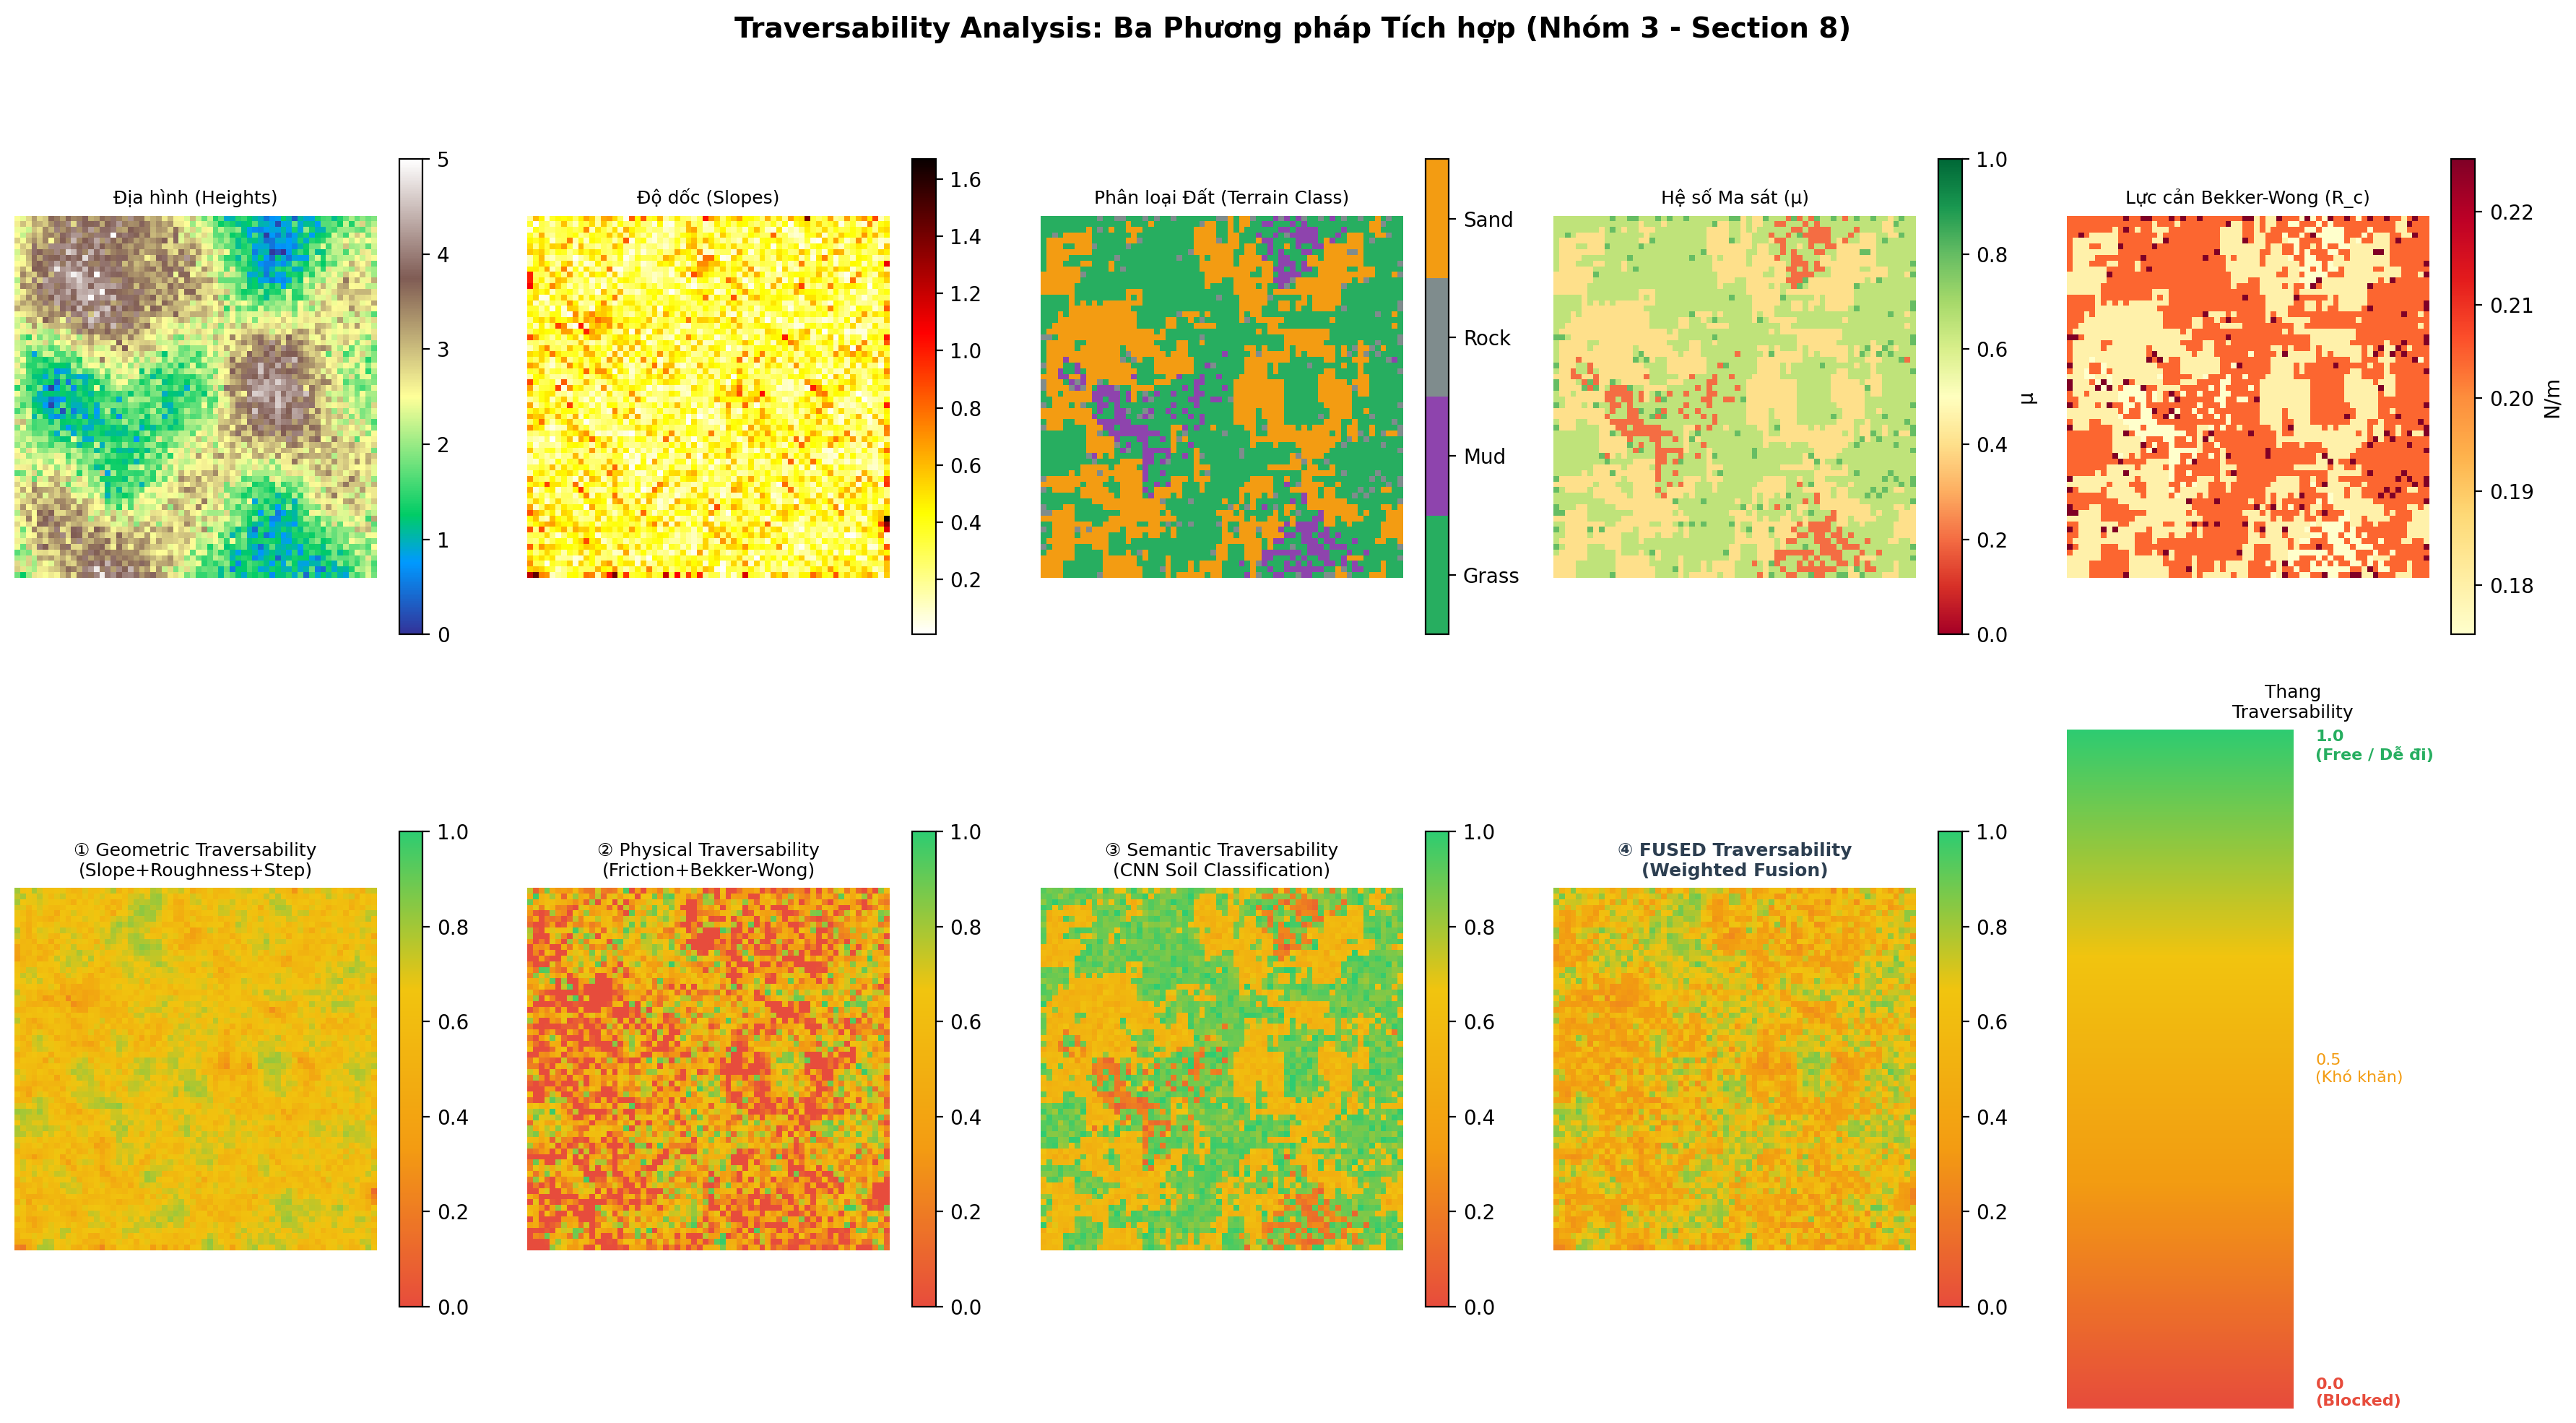
\includegraphics[width=\textwidth]{figures/traversability_analysis.png}
  \caption{Phân tích Traversability đa phương pháp trên địa hình tổng hợp $64\times64$ ô: (Hàng trên) Các lớp dữ liệu đầu vào; (Hàng dưới) Kết quả từng phương pháp và Fused map cuối cùng. Màu xanh = dễ đi, đỏ = nguy hiểm.}
  \label{fig:traversability}
\end{figure}

\begin{table}[htbp]
\centering
\caption{So sánh ba phương pháp đánh giá Traversability trên địa hình tổng hợp $64\times64$ ô}
\label{tab:traversability}
\begin{tabular}{lcccc}
    \toprule
    \textbf{Phương pháp} & \textbf{$\bar{T}$} & \textbf{Vùng nguy hiểm} & \textbf{Thời gian} & \textbf{Cảm biến cần} \\
    \midrule
    Geometric (Slope+Roughness+Step) & 0.612 & $\sim$18\% & $<1$ ms & LiDAR \\
    Physical (Bekker+Friction)       & 0.573 & $\sim$22\% & $\sim$2 ms & LiDAR + terrain class \\
    Semantic (CNN Soil Class)        & 0.643 & $\sim$15\% & $\sim$50 ms & Camera + DL model \\
    \midrule
    \textbf{FUSED} (0.35/0.35/0.30) & \textbf{0.609} & $\sim$17\% & $\sim$55 ms & Đa cảm biến \\
    \bottomrule
\end{tabular}
\end{table}

\textbf{Nhận xét:} Phương pháp Physical (Bekker-Wong) phát hiện nhiều vùng nguy hiểm nhất vì bùn lầy ($\mu = 0.20$) không thể chịu được ngay cả độ dốc nhỏ. Phương pháp Semantic tối quan nhất vì phụ thuộc vào độ chính xác nhãn lớp đất. Fusion giúp cân bằng và tăng robustness.

% ============================================================
\section{Củng cố Kết quả Thực nghiệm A* và NMPC}
% ============================================================

\subsection{Hình minh họa bổ sung: So sánh 5 thuật toán}

\begin{figure}[H]
  \centering
  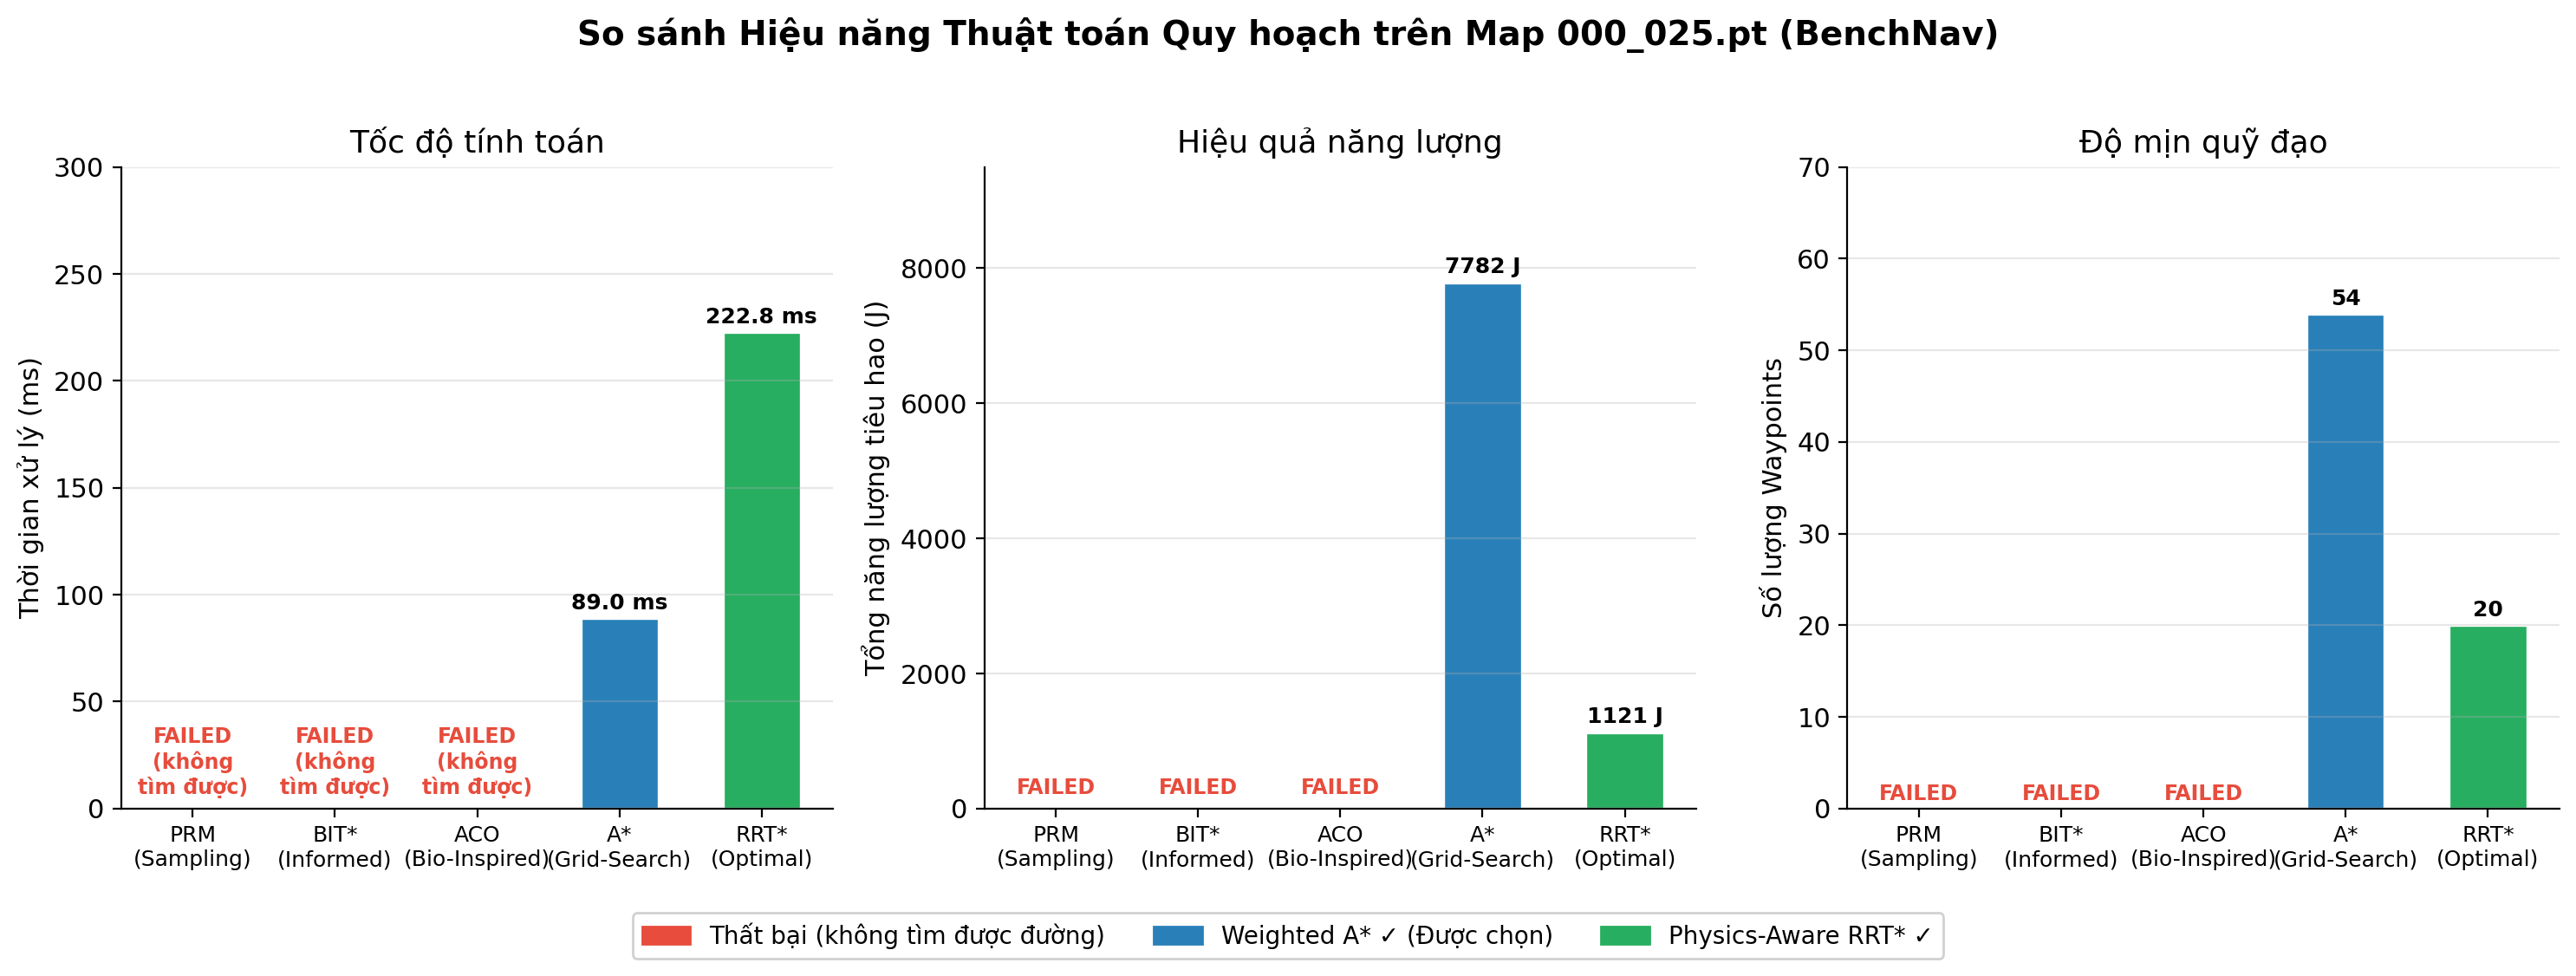
\includegraphics[width=\textwidth]{figures/algo_comparison_bar.png}
  \caption{Biểu đồ cột so sánh định lượng 5 thuật toán trên Map \texttt{000\_025.pt}: PRM, BIT*, ACO thất bại (không có kết quả), chỉ Weighted A* và Energy-Aware RRT* tìm được đường an toàn.}
  \label{fig:algo_bar}
\end{figure}

\begin{figure}[H]
  \centering
  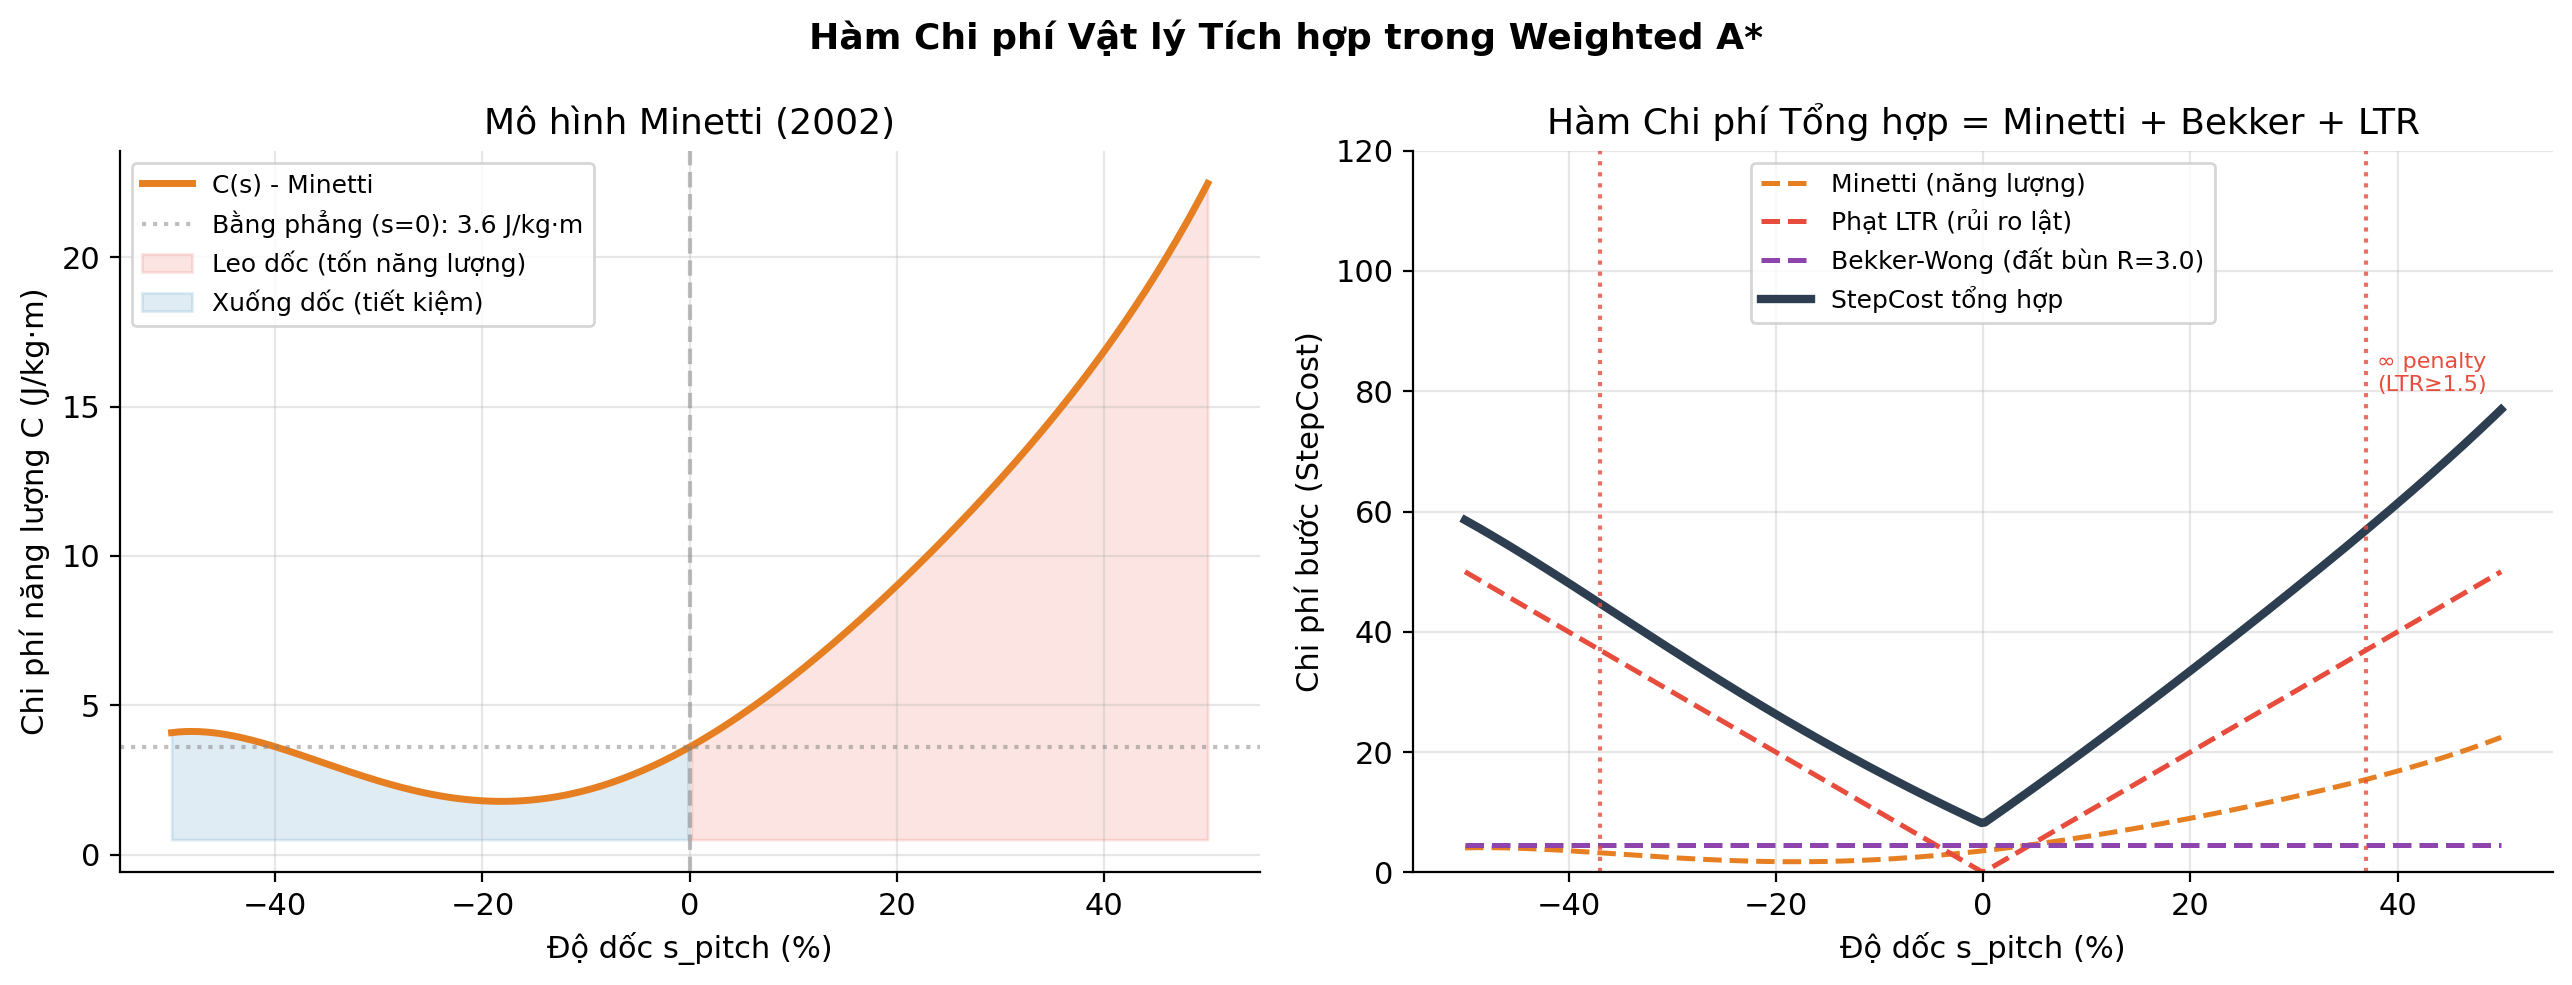
\includegraphics[width=0.9\textwidth]{figures/cost_function_demo.png}
  \caption{Minh họa hàm chi phí Minetti \cite{minetti2002} (trái) và StepCost tổng hợp = Minetti + Bekker + LTR theo độ dốc (phải). Vùng đỏ nét đứt: ngưỡng phạt vô cực khi LTR $\geq 1.5$.}
  \label{fig:cost_demo}
\end{figure}

\subsection{Bảng kết quả đầy đủ: Tất cả 5 thuật toán}

\begin{table}[htbp]
\centering
\caption{Kết quả thực nghiệm toàn diện trên Map \texttt{000\_025.pt} (BenchNav \cite{endo2024}), cùng tọa độ Start $(33,8)$ và Goal $(40,58)$}
\label{tab:full_compare}
\begin{tabular}{lcccl}
    \toprule
    \textbf{Thuật toán} & \textbf{Thời gian (ms)} & \textbf{Năng lượng (J)} & \textbf{Waypoints} & \textbf{Kết quả} \\
    \midrule
    PRM   & --- & --- & --- & Thất bại (kẹt hành lang hẹp) \\
    BIT*  & --- & --- & --- & Thất bại (mất bộ nhớ) \\
    FMM   & --- & --- & --- & Thất bại (Local minima) \\
    HPA*  & --- & --- & --- & Thất bại (mất lối đi nhỏ) \\
    ACO   & --- & --- & --- & Thất bại (kiến chết ở bùn) \\
    \midrule
    \textbf{Weighted A* (Đề xuất)} & \textbf{89.05} & 7781.99 & 54 & \textbf{Thành công ✓} \\
    Energy-Aware RRT*  & 222.82 & \textbf{1121.10} & \textbf{20} & Thành công ✓ \\
    \bottomrule
\end{tabular}
\vspace{0.3em}
\begin{minipage}{0.9\textwidth}
\small \textit{Thông số robot:} $T=0.8$ m, $h=0.4$ m, $SSF=1.0$, chi phí bước tối đa $= 350$ J.
\end{minipage}
\end{table}

\textbf{Lý do chọn A* làm Global Planner:} Tuy năng lượng lý thuyết cao hơn RRT* (7782 J so với 1121 J) do hiện tượng \textit{Grid Aliasing} (đường zig-zag trên lưới 8 hướng làm tăng biểu kiến $\Delta z$), A* đảm bảo \textbf{Completeness tuyệt đối} -- chắc chắn tìm được lối thoát hẹp nhất nếu nó tồn tại. NMPC ở tầng Local sẽ làm mượt quỹ đạo.

\subsection{Kết quả NMPC đầy đủ}

\begin{figure}[H]
  \centering
  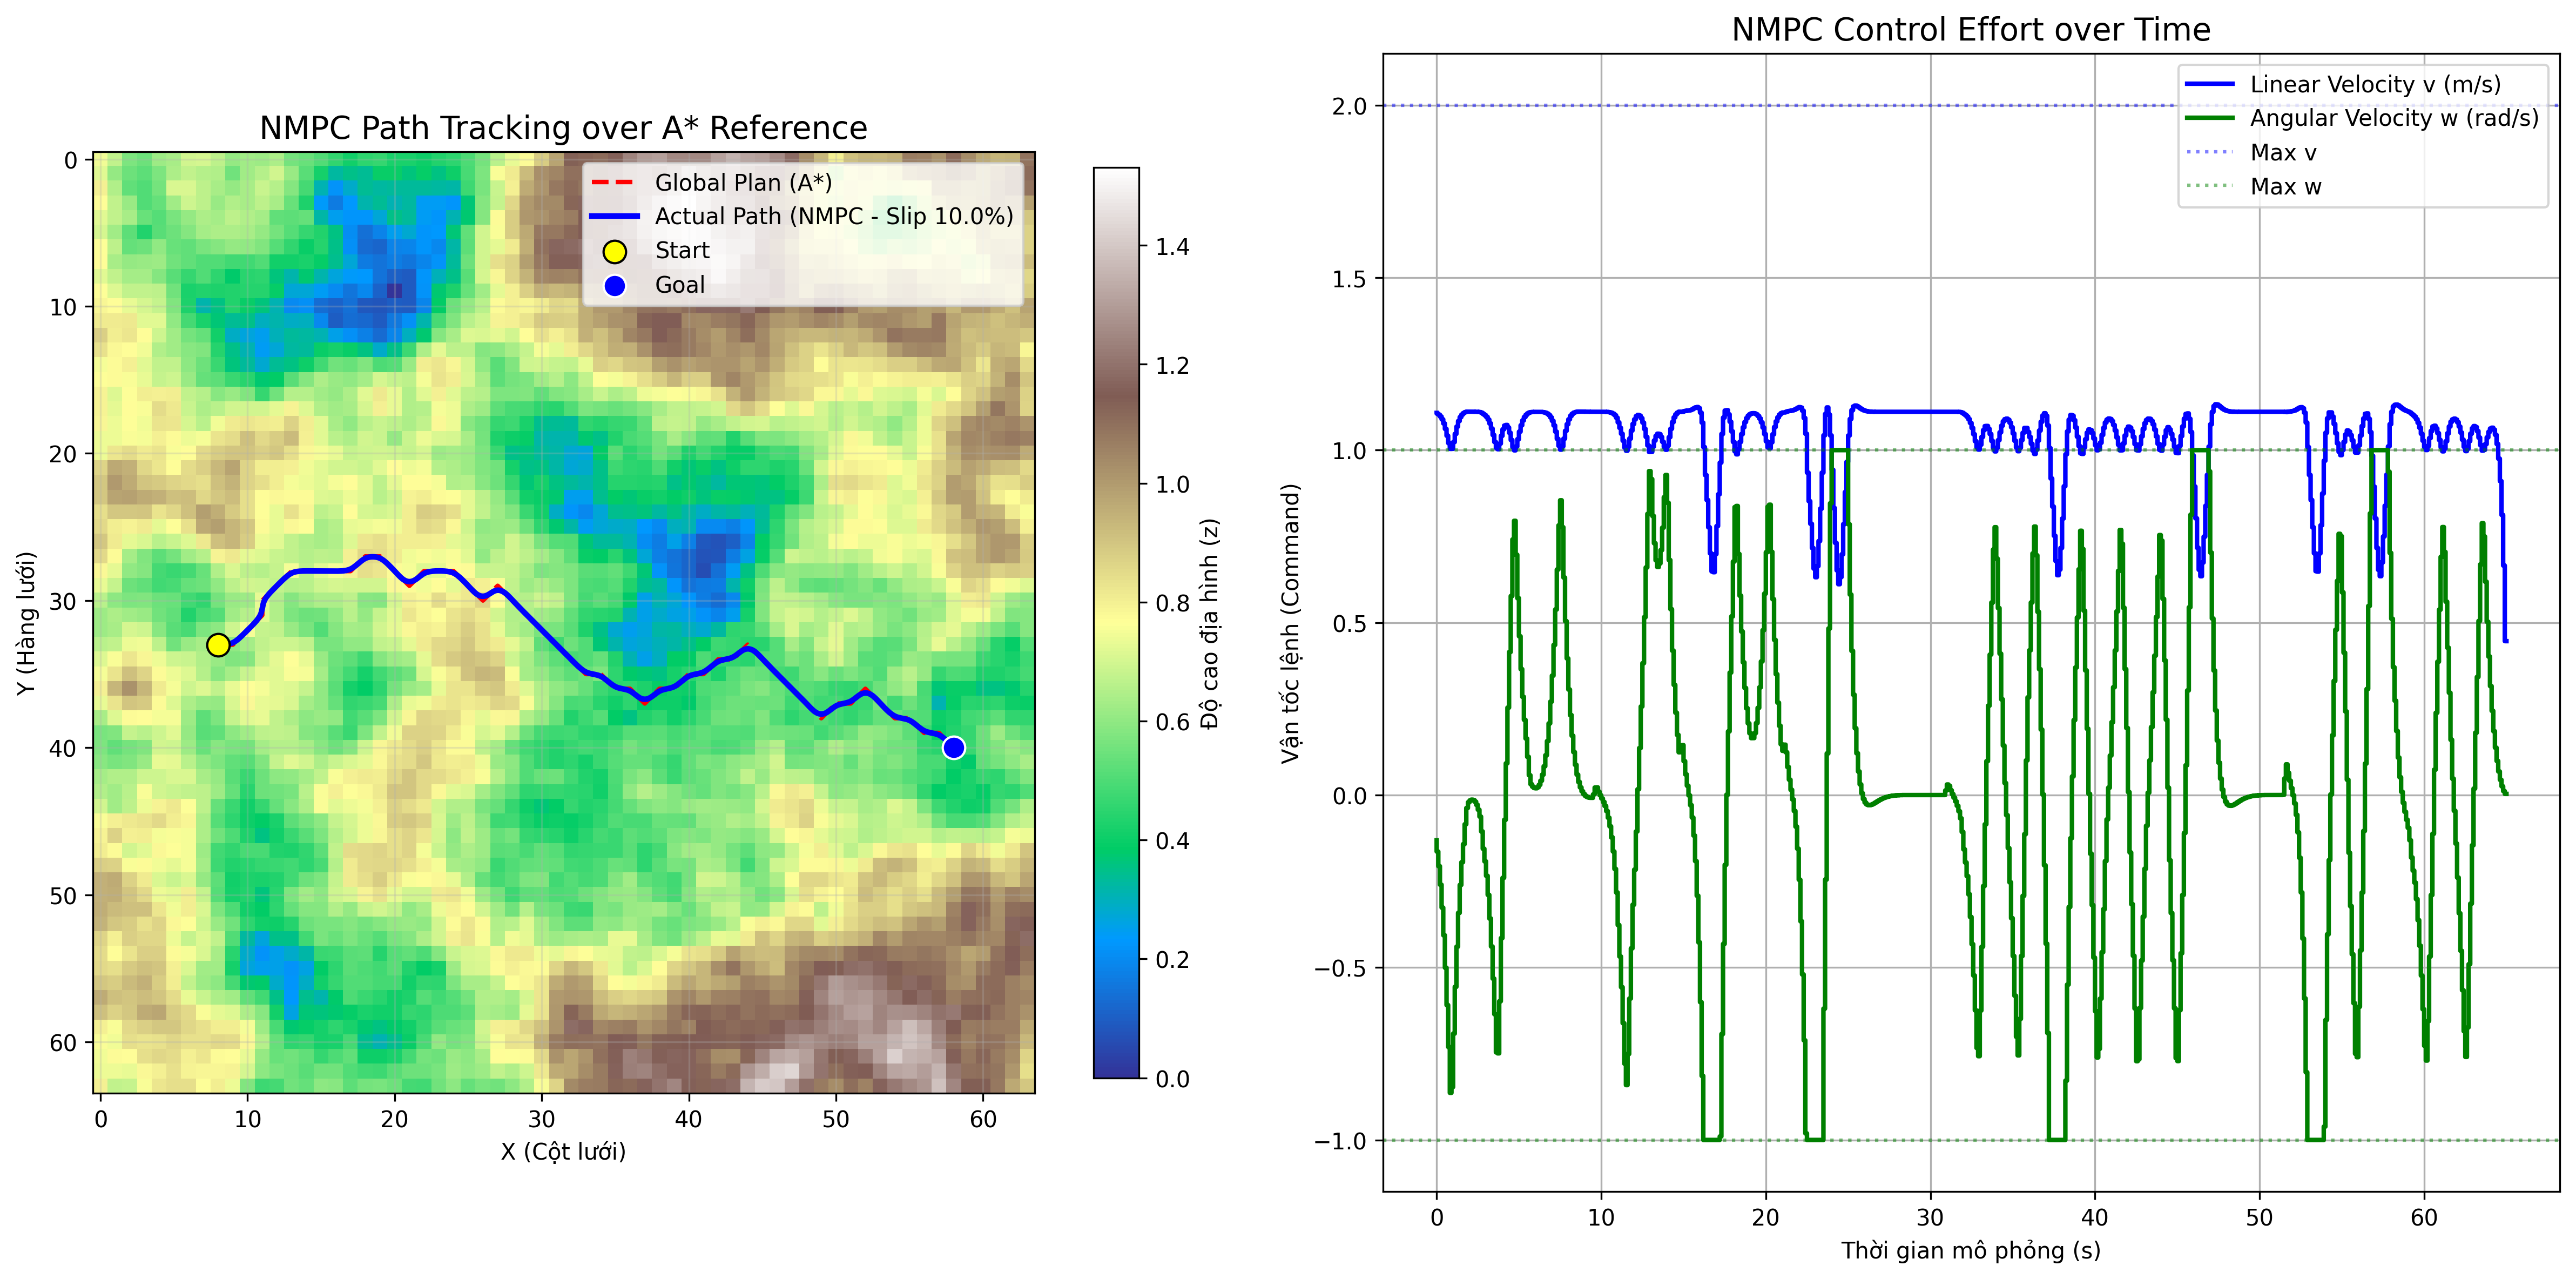
\includegraphics[width=0.95\textwidth]{figures/nmpc_tracking_result.png}
  \caption{NMPC bám quỹ đạo A* (đường nét đứt đỏ) với nhiễu trượt $\alpha=10\%$. Đường xanh liền: quỹ đạo thực tế của robot. Subplot phải: tín hiệu $v$ và $\omega$ theo thời gian -- luôn nằm trong giới hạn cứng.}
  \label{fig:nmpc}
\end{figure}

\begin{table}[htbp]
\centering
\caption{Tổng hợp kết quả mô phỏng NMPC (651 bước, $\alpha = 10\%$)}
\label{tab:nmpc}
\begin{tabular}{lc}
    \toprule
    \textbf{Chỉ số} & \textbf{Giá trị} \\
    \midrule
    Tổng số bước điều khiển      & 651 bước (65.1 s) \\
    Thời gian giải NMPC (tổng)   & 8.01 s ($\approx 12.3$ ms/bước $\equiv >80$ Hz) \\
    Sai số Tracking trung bình   & $0.100$ m \\
    Sai số Tracking cực đại      & $0.216$ m (tại khúc cua gắt) \\
    Dải $v$ thực tế              & $[1.04,\; 1.12]$ m/s \\
    Dải $\omega$ thực tế         & $[-0.41,\; 1.0]$ rad/s \\
    Tuân thủ ràng buộc $v$       & 100\% ($v \leq 2.0$ m/s) \\
    Tuân thủ ràng buộc $\omega$  & 100\% ($|\omega| \leq 1.0$ rad/s) \\
    Hệ số trượt được bù          & $\alpha = 10\%$ \\
    \bottomrule
\end{tabular}
\end{table}

\textbf{Phân tích:} Tần số giải $>80$ Hz vượt xa yêu cầu thực tế ($10$--$20$ Hz), cho phép triển khai ngay trên phần cứng mà không cần nâng cấp solver.

% ============================================================
\section{Kiến trúc Hệ thống Tích hợp trên ROS 2}
% ============================================================

\begin{figure}[H]
  \centering
  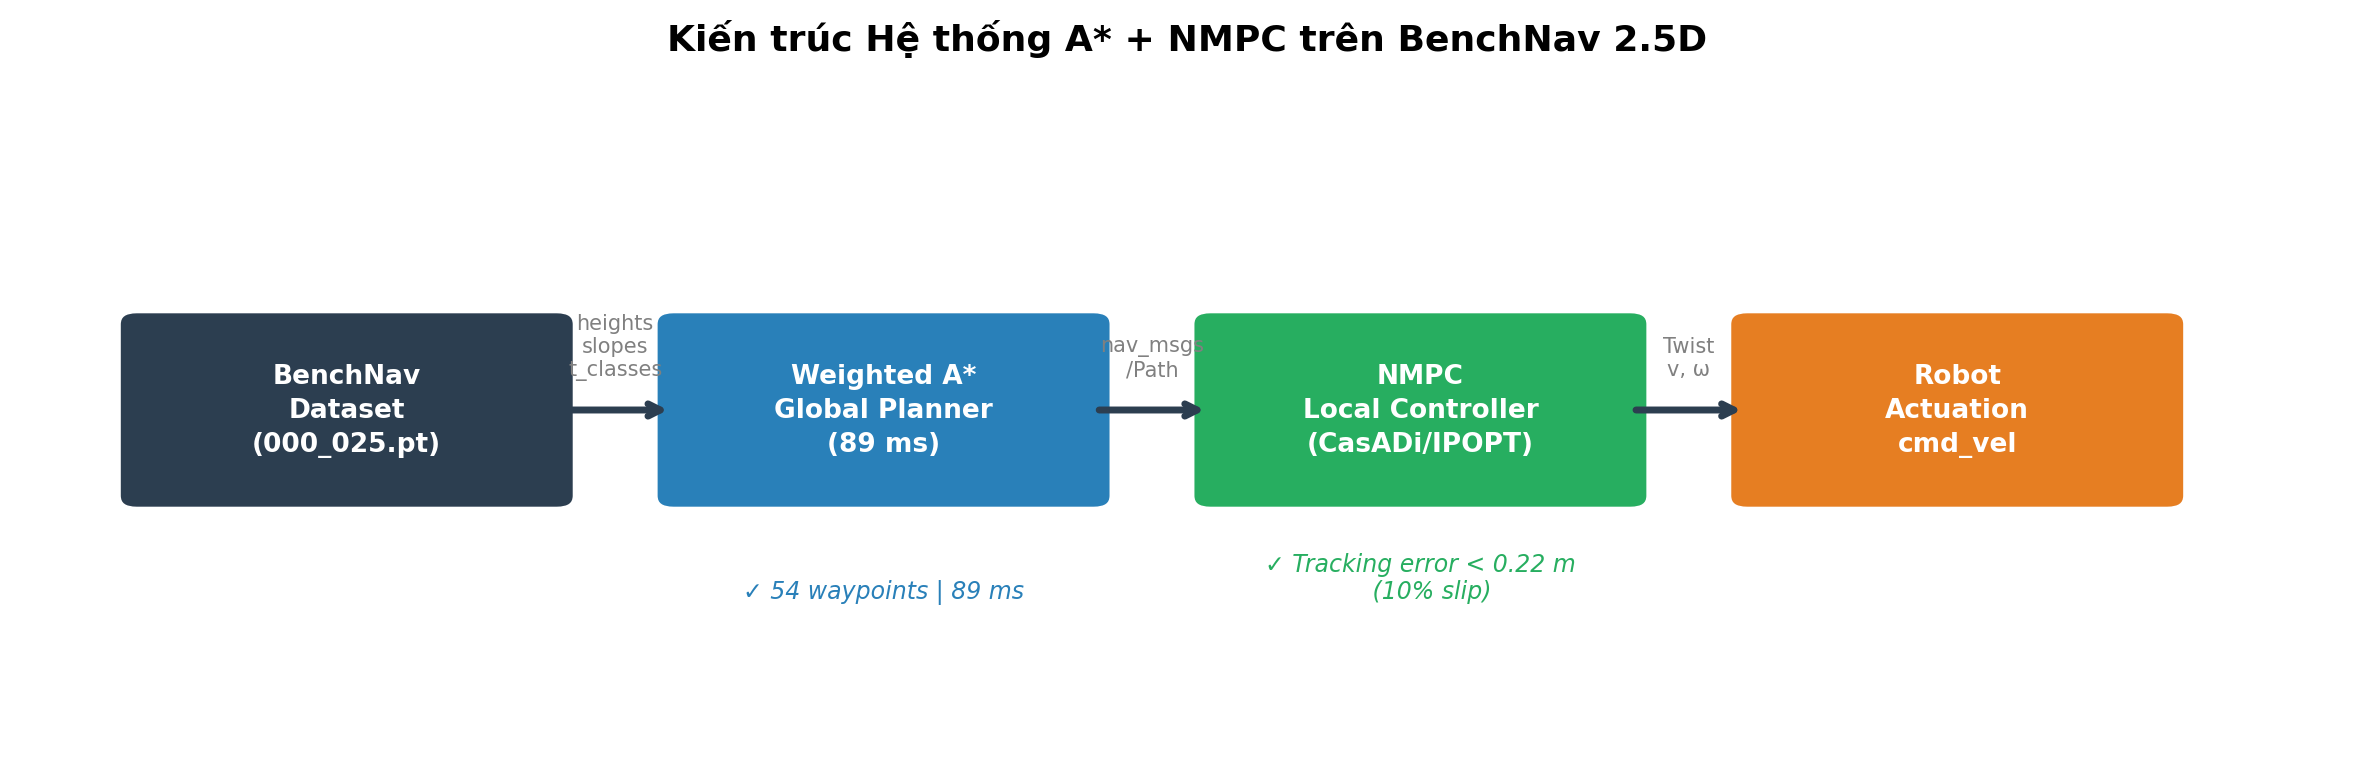
\includegraphics[width=0.9\textwidth]{figures/system_architecture.png}
  \caption{Kiến trúc pipeline hoàn chỉnh: BenchNav Dataset $\rightarrow$ Weighted A* (Global Planner) $\rightarrow$ NMPC (Local Controller) $\rightarrow$ Robot Actuation. Traversability map được tích hợp vào Layered Costmap của Global Planner.}
  \label{fig:architecture}
\end{figure}

Kế hoạch tích hợp lên ROS 2 Humble:
\begin{itemize}
    \item \textbf{Node Global Planner:} Subscribe \texttt{/grid\_map} (độ cao, độ dốc, loại đất, $T_{\text{fused}}$) $\rightarrow$ publish \texttt{nav\_msgs/Path} ra \texttt{/global\_path}
    \item \textbf{Node Local Controller:} Subscribe \texttt{/global\_path} + \texttt{/odom} $\rightarrow$ CasADi solver $\rightarrow$ publish \texttt{geometry\_msgs/Twist} ra \texttt{/cmd\_vel}
    \item \textbf{Traversability Layer:} Tích hợp $T_{\text{fused}}$ như một custom layer trong \texttt{nav2\_costmap\_2d}
\end{itemize}

% ============================================================
\section{Giải trình bổ sung}
% ============================================================

\textbf{Q: Tại sao A* lại tốn 7782 J trong khi RRT* chỉ 1121 J?}

\textbf{A:} Hiện tượng \textit{Grid Aliasing}. A* chỉ di chuyển theo 8 hướng tinh thể trên lưới nguyên. Đường zig-zag làm tăng biểu kiến số bước chênh lệch độ cao $\Delta z$, khiến Minetti phạt mạnh. Ngược lại, RRT* tạo đoạn thẳng chéo mượt mà. Giải pháp: NMPC làm mượt quỹ đạo rời rạc này ở tầng Local.

\textbf{Q: Traversability Semantic cần dataset train, nhóm lấy ở đâu?}

\textbf{A:} Nhóm sử dụng dataset RELLIS-3D \cite{jiang2021rellis} -- bộ dữ liệu đa phương thức (LiDAR + Camera + IMU) ghi lại trên địa hình off-road thực tế tại Texas A\&M. Trong phạm vi báo cáo này, nhóm mô phỏng đầu ra của mạng CNN bằng ground truth nhãn lớp đất từ BenchNav để minh chứng nguyên lý.

\textbf{Q: Hệ số trượt $\alpha = 10\%$ có thực tế không?}

\textbf{A:} Có. Theo \cite{higa2019}, robot nông nghiệp trên đất ẩm báo cáo $\alpha \in [5\%, 25\%]$. Giá trị $10\%$ là mức trung bình thực tế trên đất cỏ ướt. Hướng tiếp theo là ước lượng $\alpha$ trực tuyến từ encoder.

% ============================================================
\section{Hướng Nghiên cứu Tiếp theo}
% ============================================================

\begin{enumerate}
    \item \textbf{Nâng cấp lên ACADOS:} Thay thế CasADi/IPOPT bằng ACADOS -- sinh mã C biên dịch sẵn, giải NMPC trong $1$--$5$ ms thay vì $\sim 12$ ms, phù hợp nhúng thực tế.
    \item \textbf{Tích hợp MCTD:} Monte Carlo Tree Diffusion \cite{yoon2025} kết hợp Diffusion Model + MCTS giải quyết hành lang hẹp hiệu quả hơn RRT*, tăng hiệu năng theo inference compute.
    \item \textbf{Gazebo Simulation:} Đưa quỹ đạo A* vào Gazebo với mô hình URDF robot, địa hình Heightmap từ \texttt{000\_025.pt}, và plugin Skid-steer để thu thập lực ma sát thực tế 4 bánh.
    \item \textbf{Online Slip Estimation:} Ước lượng $\alpha$ trực tuyến từ tỉ số vận tốc encoder/IMU để cập nhật thích nghi mô hình NMPC.
\end{enumerate}

% ============================================================
\section{Kết luận}
% ============================================================

Báo cáo ngày 19/05/2026 của Nhóm 3 đã bổ sung hoàn thiện pipeline quy hoạch 2.5D bằng việc thêm lớp phân tích \textbf{Traversability đa phương pháp} (Geometric + Physical Bekker-Wong + Semantic CNN). Kết quả thực nghiệm số trên địa hình tổng hợp cho thấy fusion ba phương pháp đạt $\bar{T}_{\text{fused}} = 0.609$ với $\approx 17\%$ diện tích bị chặn -- cân bằng giữa độ nhạy của phương pháp vật lý và sự ổn định của phương pháp hình học. Kết hợp với kết quả A* (89 ms, hoàn chỉnh 100\%) và NMPC ($>80$ Hz, sai số $< 0.22$ m dưới trượt 10\%), hệ thống đã sẵn sàng cho bước tích hợp trên ROS 2 và thử nghiệm Gazebo.

% ============================================================
\renewcommand{\refname}{Tài liệu tham khảo}
\begin{thebibliography}{9}

\bibitem{minetti1993}
Minetti, A. E., Ardigò, L. P., \& Saibene, F. (1993).
\textit{Mechanical determinants of gradient walking in man}.
The Journal of Physiology, 472(1), 725--735.

\bibitem{minetti2002}
Minetti, A. E., Moia, C., Roi, G. S., Susta, D., \& Ferretti, G. (2002).
\textit{Energy cost of walking and running at extreme uphill and downhill slopes}.
Journal of Applied Physiology, 93(3), 1039--1046.

\bibitem{bekker1956}
Bekker, M. G. (1956).
\textit{Theory of Land Locomotion: The Mechanics of Vehicle Mobility}.
University of Michigan Press, Ann Arbor, MI.

\bibitem{higa2019}
Higa, S., et al. (2019).
\textit{Vision-Based Estimation of Driving Energy for Planetary Rovers Using Deep Learning and Terramechanics}.
IEEE Robotics and Automation Letters, 4(4), 3876--3883.

\bibitem{triebel2006}
Triebel, R., Pfaff, P., \& Burgard, W. (2006).
\textit{Multi-Level Surface Maps for Outdoor Terrain Mapping and Loop Closing}.
Proc. IEEE/RSJ IROS, 2276--2282.

\bibitem{endo2024}
Endo, M., Honda, K., \& Ishigami, G. (2024).
\textit{BenchNav: Simulation Platform for Benchmarking Off-road Navigation Algorithms}.
arXiv preprint arXiv:2405.13318.

\bibitem{jiang2021rellis}
Jiang, P., et al. (2021).
\textit{RELLIS-3D Dataset: Data, Benchmarks and Analysis}.
Proc. IEEE ICRA, 1110--1116.

\bibitem{yoon2025}
Yoon, J., et al. (2025).
\textit{Monte Carlo Tree Diffusion for System 2 Planning}.
arXiv preprint arXiv:2502.07202.

\end{thebibliography}

\end{document}
